\begin{enumerate}[label=\thesubsection.\arabic*.,ref=\thesubsection.\theenumi]
\numberwithin{equation}{enumi}
\item If $\vec{D}$ divides $BC$ in the ratio $k : 1$,
		\begin{align}
			\vec{D}= \frac{k\vec{C}+\vec{B}}{k+1}
	  \label{eq:section_formula}
		\end{align}
		Find the mid points $\vec{D}, \vec{E}, \vec{F}$ of the sides $BC, CA$ and $AB$ respectively.
	\\
		\solution
Since $\vec{D}$ is the midpoint of $BC$,
\begin{align}
k &= 1,\\
\implies \vec{D} &= \frac{\vec{C} + \vec{B}}{2}
= \frac{1}{2}\myvec{-7\\1}
	\label{eq:median-d}
\end{align}
Similarly,
\begin{align}
	\label{eq:median-e}
\vec{E} &= \frac{\vec{A} + \vec{C}}{2}
= \myvec{-1\\-3}\\
\vec{F} &= \frac{\vec{A} + \vec{B}}{2}
= \frac{1}{2}\myvec{-3\\5}
	\label{eq:median-f}
\end{align}
  
	\item Find the equations of $AD, BE$ and $CF$.
	\\	\\ \solution:
\begin{enumerate}
 \item The direction vector of $AD$ is 
\begin{align}
	\vec{m} = \vec{D}- \vec{A}
&=\myvec{\frac{-7}{2}\\\frac{1}{2}} - \myvec{1\\-1}
	=\frac{1}{2}\myvec{-9\\3} \equiv \myvec{-3 \\ 1}
	\\
	\implies  \vec{n} &=\myvec{1 \\ 3}
\end{align}
Hence the normal equation of median $AD$ is 
\begin{align}
\vec{n}^{\top}\myvec{\vec{x}-\vec{A}}&=0\\
\implies    \myvec{1 & 3}\vec{x}&=\myvec{1 & 3}\myvec{1\\-1}
    =-2
	\label{eq:median-ad}
\end{align}
\item For $BE$,
\begin{align}
	\vec{m}= \vec{E}- \vec{B}&=\myvec{-1\\-3} - \myvec{-4\\6}
       =\myvec{3\\-9}
       \equiv \myvec{1\\-3}
       \\
\implies 	
\vec{n} &= 
         \myvec{3\\1}
\end{align}
Hence the normal equation of median $BE$ is 
\begin{align}
\vec{n}^{\top}\myvec{\vec{x}-\vec{B}}&=0\\
\implies
	\myvec{3 & 1}   \vec{x}&=\myvec{3 &1}\myvec{-4\\6}
    =-6
	\label{eq:median-be}
\end{align}
\item For median $CF$,
\begin{align}
	\vec{m} = \vec{F}- \vec{C} &=
\myvec{\frac{-3}{2}\\\frac{5}{2}} - \myvec{-3\\-5}
       =\myvec{\frac{3}{2}\\\frac{15}{2}}
       \equiv \myvec{1 \\ 5}
       \\
	\implies \vec{n} &=\myvec{5 \\ -1}
\end{align}
Hence the normal equation of median $CF$ is 
\begin{align}
\vec{n}^{\top}\myvec{\vec{x}-\vec{C}}&=0\\
	\implies \myvec{5 & -1}\vec{x}&=\myvec{5 & -1}\myvec{-3\\-5}
    =-10
	\label{eq:median-cf}
\end{align}
\end{enumerate}
\iffalse
\begin{figure}
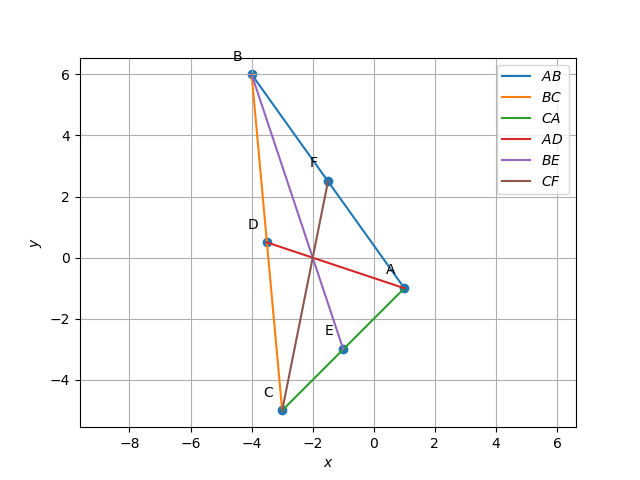
\includegraphics [width=\columnwidth] {solutions/1/2/2/figs/figure.png}
\caption{ Medians $AD$ , $BE$ and $CF$}
\label{fig: medians}
\end{figure}
\fi




% 		\iffalse
\let\negmedspace\undefined
\let\negthickspace\undefined
\documentclass[journal,12pt,twocolumn]{IEEEtran}
\usepackage{cite}
\usepackage{amsmath,amssymb,amsfonts,amsthm}
\usepackage{algorithmic}
\usepackage{graphicx}
\usepackage{textcomp}
\usepackage{xcolor}
\usepackage{txfonts}
\usepackage{listings}
\usepackage{enumitem}
\usepackage{mathtools}
\usepackage{gensymb}
\usepackage[breaklinks=true]{hyperref}
\usepackage{tkz-euclide} % loads  TikZ and tkz-base
\usepackage{listings}
\usepackage{gvv}
%
%\usepackage{setspace}
%\usepackage{gensymb}
%\doublespacing
%\singlespacing

%\usepackage{graphicx}
%\usepackage{amssymb}
%\usepackage{relsize}
%\usepackage[cmex10]{amsmath}
%\usepackage{amsthm}
%\interdisplaylinepenalty=2500
%\savesymbol{iint}
%\usepackage{txfonts}
%\restoresymbol{TXF}{iint}
%\usepackage{wasysym}
%\usepackage{amsthm}
%\usepackage{iithtlc}
%\usepackage{mathrsfs}
%\usepackage{txfonts}
%\usepackage{stfloats}
%\usepackage{bm}
%\usepackage{cite}
%\usepackage{cases}
%\usepackage{subfig}
%\usepackage{xtab}
%\usepackage{longtable}
%\usepackage{multirow}
%\usepackage{algorithm}
%\usepackage{algpseudocode}
%\usepackage{enumitem}
%\usepackage{mathtools}
%\usepackage{tikz}
%\usepackage{circuitikz}
%\usepackage{verbatim}
%\usepackage{tfrupee}
%\usepackage{stmaryrd}
%\usetkzobj{all}
%    \usepackage{color}                                            %%
%    \usepackage{array}                                            %%
%    \usepackage{longtable}                                        %%
%    \usepackage{calc}                                             %%
%    \usepackage{multirow}                                         %%
%    \usepackage{hhline}                                           %%
%    \usepackage{ifthen}                                           %%
  %optionally (for landscape tables embedded in another document): %%
%    \usepackage{lscape}     
%\usepackage{multicol}
%\usepackage{chngcntr}
%\usepackage{enumerate}

%\usepackage{wasysym}
%\documentclass[conference]{IEEEtran}
%\IEEEoverridecommandlockouts
% The preceding line is only needed to identify funding in the first footnote. If that is unneeded, please comment it out.

\newtheorem{theorem}{Theorem}[section]
\newtheorem{problem}{Problem}
\newtheorem{proposition}{Proposition}[section]
\newtheorem{lemma}{Lemma}[section]
\newtheorem{corollary}[theorem]{Corollary}
\newtheorem{example}{Example}[section]
\newtheorem{definition}[problem]{Definition}
%\newtheorem{thm}{Theorem}[section] 
%\newtheorem{defn}[thm]{Definition}
%\newtheorem{algorithm}{Algorithm}[section]
%\newtheorem{cor}{Corollary}
\newcommand{\BEQA}{\begin{eqnarray}}
\newcommand{\EEQA}{\end{eqnarray}}
\newcommand{\define}{\stackrel{\triangle}{=}}
\theoremstyle{remark}
\newtheorem{rem}{Remark}

%\bibliographystyle{ieeetr}
\begin{document}
%

\bibliographystyle{IEEEtran}


\vspace{3cm}

\title{ Solution of 1.2.2
%	\logo{

%	}
}
\author{ Dhruv Parashar$^{*}$% <-this % stops a space
	
}	
%\title{
%	\logo{Matrix Analysis through Octave}{\begin{center}\includegraphics[scale=.24]{tlc}\end{center}}{}{HAMDSP}
%}


% paper title
% can use linebreaks \\ within to get better formatting as desired
%\title{Matrix Analysis through Octave}
%
%
% author names and IEEE memberships
% note positions of commas and nonbreaking spaces ( ~ ) LaTeX will not break
% a structure at a ~ so this keeps an author's name from being broken across
% two lines.
% use \thanks{} to gain access to the first footnote area
% a separate \thanks must be used for each paragraph as LaTeX2e's \thanks
% was not built to handle multiple paragraphs
%

%\author{<-this % stops a space
%\thanks{}}
%}
% note the % following the last \IEEEmembership and also \thanks - 
% these prevent an unwanted space from occurring between the last author name
% and the end of the author line. i.e., if you had this:
% 
% \author{....lastname \thanks{...} \thanks{...} }
%                     ^------------^------------^----Do not want these spaces!
%
% a space would be appended to the last name and could cause every name on that
% line to be shifted left slightly. This is one of those "LaTeX things". For
% instance, "\textbf{A} \textbf{B}" will typeset as "A B" not "AB". To get
% "AB" then you have to do: "\textbf{A}\textbf{B}"
% \thanks is no different in this regard, so shield the last } of each \thanks
% that ends a line with a % and do not let a space in before the next \thanks.
% Spaces after \IEEEmembership other than the last one are OK (and needed) as
% you are supposed to have spaces between the names. For what it is worth,
% this is a minor point as most people would not even notice if the said evil
% space somehow managed to creep in.



% The paper headers
%\markboth{Journal of \LaTeX\ Class Files,~Vol.~6, No.~1, January~2007}%
%{Shell \MakeLowercase{\textit{et al.}}: Bare Demo of IEEEtran.cls for Journals}
% The only time the second header will appear is for the odd numbered pages
% after the title page when using the twoside option.
% 
% *** Note that you probably will NOT want to include the author's ***
% *** name in the headers of peer review papers.                   ***
% You can use \ifCLASSOPTIONpeerreview for conditional compilation here if
% you desire.




% If you want to put a publisher's ID mark on the page you can do it like
% this:
%\IEEEpubid{0000--0000/00\$00.00~\copyright~2007 IEEE}
% Remember, if you use this you must call \IEEEpubidadjcol in the second
% column for its text to clear the IEEEpubid mark.



% make the title area
\maketitle

\newpage

%\tableofcontents

\bigskip

\renewcommand{\thefigure}{\theenumi}
\renewcommand{\thetable}{\theenumi}
%\renewcommand{\theequation}{\theenumi}

%\begin{abstract}
%%\boldmath
%In this letter, an algorithm for evaluating the exact analytical bit error rate  (BER)  for the piecewise linear (PL) combiner for  multiple relays is presented. Previous results were available only for upto three relays. The algorithm is unique in the sense that  the actual mathematical expressions, that are prohibitively large, need not be explicitly obtained. The diversity gain due to multiple relays is shown through plots of the analytical BER, well supported by simulations. 
%
%\end{abstract}
% IEEEtran.cls defaults to using nonbold math in the Abstract.
% This preserves the distinction between vectors and scalars. However,
% if the journal you are submitting to favors bold math in the abstract,
% then you can use LaTeX's standard command \boldmath at the very start
% of the abstract to achieve this. Many IEEE journals frown on math
% in the abstract anyway.

% Note that keywords are not normally used for peerreview papers.
%\begin{IEEEkeywords}
%Cooperative diversity, decode and forward, piecewise linear
%\end{IEEEkeywords}



% For peer review papers, you can put extra information on the cover
% page as needed:
% \ifCLASSOPTIONpeerreview
% \begin{center} \bfseries EDICS Category: 3-BBND \end{center}
% \fi
%
% For peerreview papers, this IEEEtran command inserts a page break and
% creates the second title. It will be ignored for other modes.
%\IEEEpeerreviewmaketitle


Question:- 
We are given the three vertices of a triangle$(A,B,C)$ and the midpoints $\vec{D},\vec{E},\vec{F}$ of the sides $AB,BC,AC$ respectively. We have to find the equations of the sides $AD,BE,CF$.
\\
\fi
\solution
\begin{align}
\vec{A} &= \myvec{1\\-1} \\
\vec{B} &= \myvec{-4\\6} \\
\vec{C} &= \myvec{-3\\-5}
\end{align}
The mid points $\vec{D},\vec{E},\vec{F}$ of sides $AB,BC,AC$ are :-
\begin{align}
\vec{D} &= \frac{1}{2}\myvec{-7  \\ 1}\\
\vec{E} &= \myvec{-1\\-3}\\
\vec{F} &= \frac{1}{2}\myvec{-3  \\ 5}
\end{align}
Now, the direction vector of line $FC(\vec{m})$ is :-
\begin{align}
\vec{m} &= \vec{F} - \vec{C} \\
\implies \vec{m} &= \frac{1}{2}\myvec{3 \\ 15}
\end{align}
Now, we have to find $\vec{n}$,
\begin{align}
\vec{n} &= \myvec{0 & 1 \\ -1 & 0}\vec{m}\\
&= \frac{1}{2}\myvec{0 & 1 \\ -1 & 0}\myvec{3\\15}\\
&=\frac{1}{2}\myvec{15\\-3}
\end{align}
Normal form of line CF is :
\begin{align}
\vec{n}^{\top}(\vec{x-C}) &= 0\\
\vec{n}^{\top}\vec{x} &= \vec{n}^{\top}\vec{C} \\
\frac{1}{2}\myvec{15 & -3}\vec{x} &= \frac{1}{2}\myvec{15 & -3}\myvec{-3\\-5} \\
\myvec{15 & -3}\vec{x} &= \myvec{15 & -3}\myvec{-3\\-5} \\
\myvec{15 & -3}\vec{x} &= -30
\end{align}

\begin{figure}
\centering
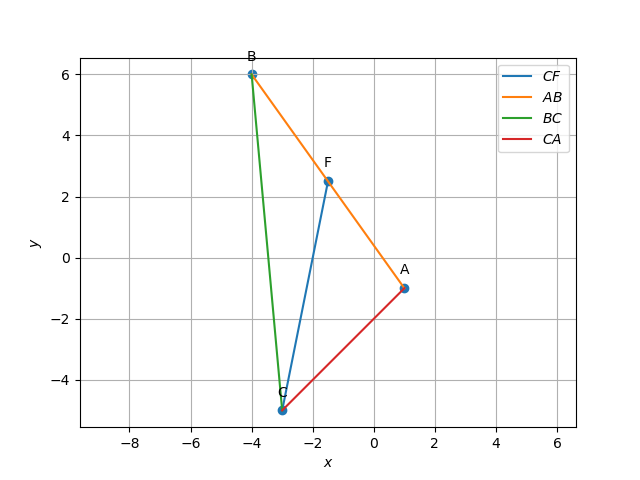
\includegraphics[width=\columnwidth]{solutions/1/2/2a/figs/figure.png}
\caption{Line CF}
\label{fig:Line CF}
\end{figure}



	\item Find the intersection $\vec{G}$ of $BE$ and $CF$.
 \\
\solution 
From 
	\eqref{eq:median-be}
	and
	\eqref{eq:median-cf},
the equations of $BE$ 
and 
$CF$
are, respectively,
\begin{align}
\myvec{3 & 1} \vec{x} &= \myvec{-6}
\label{eq:1.2.3,8}
\\
\myvec{ 5&-1} \vec{x} &= \myvec{-10}
\label{eq:1.2.3,9}
\end{align}
From \eqref{eq:1.2.3,8} and \eqref{eq:1.2.3,9} the augmented matrix is
\begin{align}
    \label{eq:matrowoperations}
    \myvec{
    3 & 1 & -6
    \\
    5 & -1 & -10
    }
     \xleftrightarrow[]{R_1 \leftarrow R_1+R_2}
    \myvec{
    8 & 0 & -16
    \\
    5 & -1 & -10 
    }
    \\
     \xleftrightarrow[]{R_1\leftarrow R_1/8}
    \myvec{
    1 & 0 & -2
    \\
    5 & -1 & -10 
    }
     \xleftrightarrow[]{R_2\leftarrow R_2-5R_1}
    \myvec{
    1 & 0 & -2
    \\
    0 & -1 & 0
    }
    \\
     \xleftrightarrow[]{R_2\leftarrow -R_2}
    \myvec{
    1 & 0 & -2
    \\
    0 & 1 & 0
    }
\end{align} 
using Gauss elimination.  Therefore, 
\begin{align}
\vec{G} = \myvec{-2 \\ 0}
	\label{eq:median-g}
\end{align}

	\item Verify that 
		\begin{align}
			\frac{BG}{GE} = 
			\frac{CG}{GF} =
			\frac{AG}{GD} =2 
		\end{align}
		\\	\solution 
\begin{enumerate}
\item From 
	\eqref{eq:median-e}
	and
	\eqref{eq:median-g},
\begin{align}
		\label{eq:tri-pts/4} \vec{G}-\vec{B} &= \myvec{2 \\ -6},\, 
 \vec{E}-\vec{G} = \myvec{1 \\ -3} \\
	\implies \vec{G}-\vec{B} &= 2 \brak{ \vec{E}-\vec{G} }
	\\
	\implies \norm{\vec{G}-\vec{B}} &= 2 \norm{ \vec{E}-\vec{G} }
	\\
	\text{or, }		\label{eq:tri-pts/8}\frac{BG}{GE} &=  2  
\end{align}		
\item From 
	\eqref{eq:median-f}
	and
	\eqref{eq:median-g},
\begin{align}
		 \vec{F}-\vec{G} &= \frac{1}{2}\myvec{ 1 \\ 5},\, 
 \vec{G}-\vec{C} &= \myvec{1 \\ 5} \\
	\implies 		 \vec{G}-\vec{C} &= 2 \brak{\vec{F}-\vec{G}} 
	\\
	\implies 		 \norm{\vec{G}-\vec{C}} &= 2 \norm{\vec{F}-\vec{G}} 
	\\
		\text{or, }	\frac{CG}{GF} &=  2		
\label{eq:tri-pts/9}
\end{align}
\item From
	\eqref{eq:median-d}
	and
	\eqref{eq:median-g},
\begin{align}
		\label{eq:tri-pts/14} \vec{G}-\vec{A} &= \myvec{-3 \\ 1} ,\,
 \vec{D}-\vec{G} = \frac{1}{2}\myvec{ -3 \\ 1}
 \\
	\vec{G}-\vec{A} &= 
	2\brak{ \vec{D}-\vec{G} } 
	\\
\implies		 \norm{\vec{G}-\vec{A}} &= 
 2\norm{\vec{D}-\vec{G}} 
 \\
		\text{or, }		\label{eq:tri-pts/18}\frac{AG}{GD} &=   2		
\end{align}
\end{enumerate}
From \eqref{eq:tri-pts/8}, \eqref{eq:tri-pts/9}, \eqref{eq:tri-pts/18}
\begin{align}
		\frac{BG}{GE} = 
		\frac{CG}{GF} =
		\frac{AG}{GD} = 2
\end{align}

	\item Show that $\vec{A}, \vec{G}$ and $\vec{D}$ are collinear.
	\\
		\solution 
Points $\vec{A},\vec{D},\vec{G}$ are defined to be collinear if 
\begin{align}
    \text{rank}\myvec{
    1 & 1 & 1\\
    \vec{A} & \vec{D} & \vec{G} \\
    } = 2 
    \label{eq:mat_row_operations}
    \\
\implies    
    \myvec{
    1 & 1 & 1
    \\
    1 & -\frac{7}{2} & -2
    \\
    -1 & \frac{1}{2} & 0
    }
     \xleftrightarrow[]{R_3 \leftarrow R_3+R_2}
    \myvec{
    1 & 1 & 1
    \\
    1 & -\frac{7}{2} & -2
    \\
    0 & -3 & -2 
    }
    \\
     \xleftrightarrow[]{R_2\leftarrow R_2-R_1}
    \myvec{
    1 & 1 & 1
    \\
    0 & -\frac{9}{2} & -3
    \\
    0 & -3 & -2 
    }
     \xleftrightarrow[]{R_3\leftarrow R_3-\frac{2}{3}R_2}
    \myvec{
    1 & 1 & 1
    \\
    0 & -\frac{9}{2} & -3
    \\
    0 & 0 & 0
    }
\end{align}
Thus, the matrix 
    \eqref{eq:mat_row_operations}
    has rank 2 and the points are collinear.
    Thus, the medians of a triangle meet at the point $\vec{G}$.
See \figref{fig:Triangle-median}.
\begin{figure}
\centering
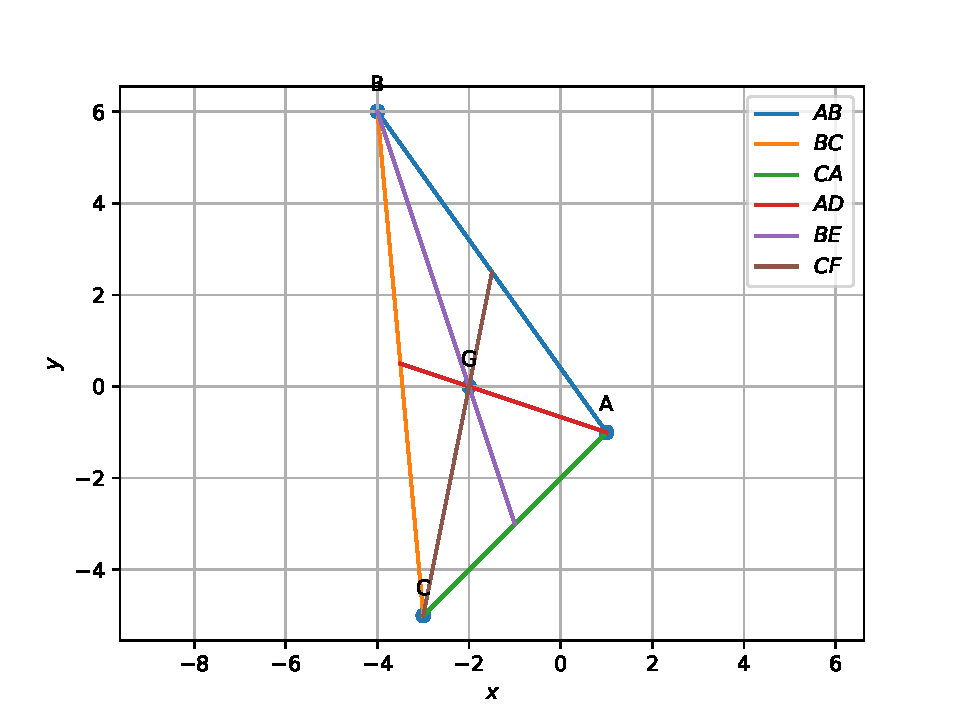
\includegraphics[width=\columnwidth]{figs/triangle/median.pdf}
	\caption{Medians of $\triangle ABC$ meet at $\vec{G}$.}
\label{fig:Triangle-median}
\end{figure}


	\item Verify that 
		\begin{align}
			\vec{G}=\frac{\vec{A}+\vec{B}+\vec{C}}{3}
		\end{align}
			$\vec{G}$ is known as the {\em centroid} of $\triangle ABC$.
   \\
		\solution
\begin{equation}
\begin{split}
\label{eq:centroid}
    \vec{G}&= \frac{\myvec{1\\-1}+\myvec{-4\\6}+\myvec{-3\\-5}}{3}\\    
     &= \myvec{-2\\0}
\end{split}
\end{equation}

 




	\item Verify that 
		\begin{align}
\vec{A}-\vec{F}=\vec{E}-\vec{D}
		\end{align}
		The quadrilateral $AFDE$ is defined to be a parallelogram.\\
  		\\ \solution 
\begin{align}
    \vec{A}-\vec{F}&=\myvec{1\\-1}-\myvec{\frac{-3}{2}\\\frac{5}{2}}
    =\myvec{\frac{5}{2}\\\frac{-7}{2}}
    \\
    \vec{E}-\vec{D}&=\myvec{-1\\-3}-\myvec{\frac{-7}{2}\\\frac{1}{2}}
    =\myvec{\frac{5}{2}\\\frac{-7}{2}}
    \\
	\implies	\vec{A}-\vec{F} &= \vec{E}-\vec{D}
\end{align}
See \figref{fig:Triangle-pgm}, 
\begin{figure}
\centering
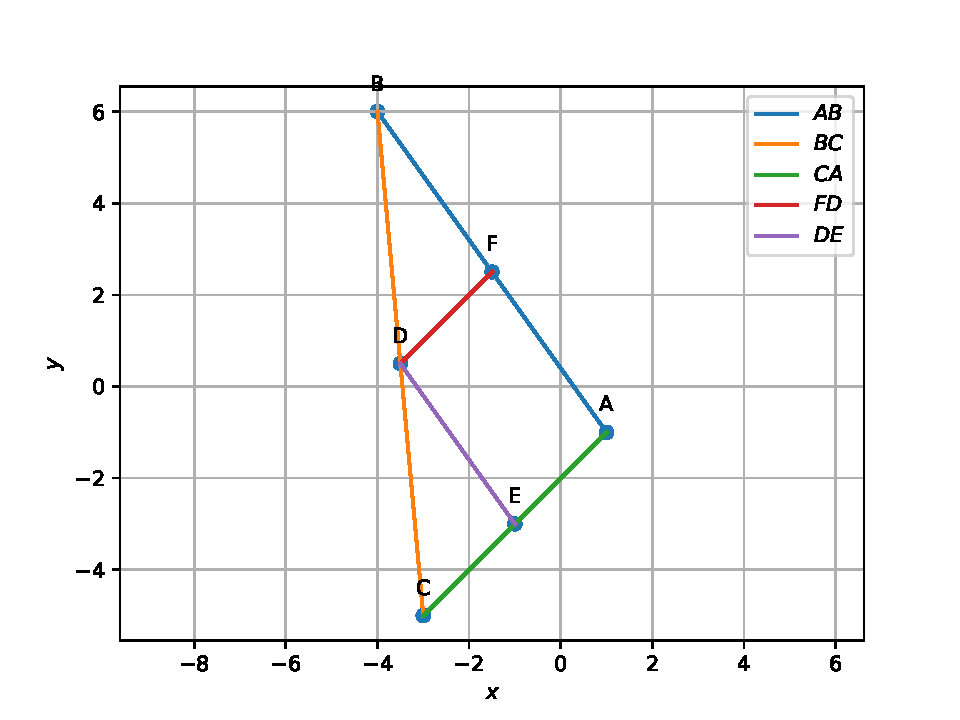
\includegraphics[width=\columnwidth]{figs/triangle/pgm.pdf}
\caption{$AFDE$ forms a parallelogram in triangle ABC}
\label{fig:Triangle-pgm}
\end{figure}






















All codes for this section are available in 
\begin{lstlisting}
	codes/triangle/medians.py
	codes/triangle/pgm.py
\end{lstlisting}
  
\end{enumerate}
